\documentclass[a4paper,12pt, titlepage]{article}
\usepackage[ngerman]{babel}
\usepackage[left = 2cm, right = 2cm, top = 2cm, bottom = 2cm]{geometry}
\usepackage{graphicx}
\usepackage{hyperref}
\setlength{\parindent}{0cm}
\usepackage{setspace}
\usepackage{titlesec}
\usepackage{listings}
\usepackage{tocloft}
\usepackage{minted}
\usepackage{fancyhdr}

\renewcommand{\listingscaption}{Auflistung}
\renewcommand{\listoflistingscaption}{Quellcodeverzeichnis}


\usepackage{xcolor}
\definecolor{LightGray}{gray}{0.9} % background

\titleformat*{\section}{\Huge\bfseries}



\begin{document}
\setlength\parindent{0cm}


\begin{titlepage}
	
\includegraphics[scale = 0.6]{HSBochum-logo.png}

	\vspace{2cm}
	{
		\begin{center}
			\LARGE\textbf{Fachbereich Elektrotechnik und Informatik}\\
			\vspace{0.3cm}
			\textbf{Erweiterte Programmiersprachen}\\
			\vspace{0.3cm}
			\textbf{SS24}\\
			\vspace{1cm}
			\LARGE\textit{\glqq{Prognose der von aussterben bedrohten Bevölkerung Chinas im Jahr 2100 mit Julia}\grqq }\\
			\vspace{1cm}
			\large{zur Erlangung des Grades\\}
			\textbf{Bachelor of Science}
		\end{center}
	}

	\vspace{3cm}
	{
		\large\textbf{Vorgelegt von Emre Akarsu\\}
		\normalsize{Matrikelnummer: 018345607}\\
		\href{mailto: emre.akarsu@stud.hs-bochum.de}{Emre.akarsu@stud.hs-bochum.de}
		\\
		Studiengang: Bachelor Informatik\\
		Fachsemester: 6
	}

	\vspace{3cm}
	{
		\begin{tabular}{@{}ll}
			Abzugeben an:
		\end{tabular}
		\begin{tabular}{@{}ll}
			Prof. Dr.-Ing. Edmund Coersmeier
		\end{tabular}
	}
	\\Abgabedatum: \today
\end{titlepage}



\onehalfspacing
\newpage
\pagenumbering{gobble}
\pagestyle{empty}
\tableofcontents
\newpage
\pagestyle{plain}
\pagenumbering{roman}
\addcontentsline{toc}{section}{Abbildungsverzeichnis}
% Input: Abbildungsverzeichnis
\listoffigures
\setcounter{page}{1}
\newpage



% Quellcodeverzeichnis
\newpage
\listoflistings
\newpage


\setcounter{page}{1}
\newpage
\pagenumbering{arabic}

\renewcommand{\headrulewidth}{0pt}
\newpage

\renewcommand{\headrulewidth}{0.4pt}
\pagestyle{fancy}
\fancyhead[L]{\textit{Hochschule Bochum}}
\fancyhead[C]{Erweiterte Programmiersprachen}
\fancyhead[R]{\textit{Emre Akarsu}}


\section{Einleitung}
China ist das bevölkerungsreichste Land der Welt und spielt eine zentrale Rolle in der globalen Demografie. In den letzten Jahrzehnten hat das Land jedoch eine signifikante demografische Verschiebung erlebt, die durch eine alternde Bevölkerung und eine niedrige Geburtenrate gekennzeichnet ist. Die ein Kind Politik, die von 1979 bis 2015 in China in Kraft war, hat zu einem Ungleichgewicht zwischen den Geschlechtern und einer alternden Bevölkerung geführt. Lebenshaltungskosten und wirtschaftliche Unsicherheit haben auch dazu beigetragen, dass viele Paare sich gegen Kinder entscheiden. Diese demografischen Herausforderungen könnten langfristige Auswirkungen auf die wirtschaftliche und soziale Entwicklung Chinas haben.\\  

Unter berücksichtigung dieser Aspekte ist es von entscheidender Bedeutung, die demografische Entwicklung Chinas zu analysieren und Prognosen für die Zukunft zu erstellen.\\

Dieses Projekt zielt darauf ab, die demografische Entwicklung Chinas bis zum Jahr 2100 zu modellieren und zu analysieren. Dazu verwenden wir die Programmiersprache Julia, die sich durch ihre Leistungsfähigkeit und Effizienz bei der Verarbeitung großer Datenmengen auszeichnet. 
\\


\subsection{Problemstellung}
China steht vor einer demografischen Herausforderung, die tiefgreifende Auswirkungen auf die wirtschaftliche und soziale Struktur des Landes hat. Die Hauptprobleme sind:


\begin{enumerate}
\item Sinkende Geburtenrate: Die Geburtenrate in China ist seit Jahrzehnten rückläufig und liegt mittlerweile weit unter dem für den Bevölkerungsersatz notwendigen Niveau.
\item Alternde Bevölkerung: Der Anteil älterer Menschen in der chinesischen Gesellschaft nimmt stetig zu, was zu einer erhöhten Belastung des Rentensystems und des Gesundheitswesens führt.
%\item Niedrige Migrationsrate: Die Netto-Migration kann den Bevölkerungsrückgang nicht ausgleichen, da China historisch gesehen wenig Zuwanderung verzeichnet.
%\item Ungleichmäßige regionale Verteilung: Die Bevölkerungsdichte in China variiert stark zwischen den städtischen und ländlichen Gebieten, was zu sozialen und wirtschaftlichen Disparitäten führt.
\item Ein-Kind-Politik: Obwohl die Ein-Kind-Politik in China offiziell abgeschafft wurde, hat sie langfristige Auswirkungen auf die Bevölkerungsstruktur des Landes.
\item Zu hohe Lebenshaltungskosten: Das verfügbare Einkommen und die Lebenshaltungskosten haben einen direkten Einfluss auf die Familienplanung und die Geburtenrate in China.
\end{enumerate}
Diese Probleme führen zu einem erwarteten Bevölkerungsrückgang, der die wirtschaftliche Stabilität und das soziale Wohlergehen Chinas bedrohen könnte.

\subsection{Methodik und Strategie}

Die für diese Hausarbeit verwendeten Daten stammen aus verschiedenen Quellen, darunter:
\begin{itemize}
\item Bevölkerungsstatistiken der Vereinten Nationen (UN)
\item National Bureau of Statistics of China (NBS)
\item WorldPop Datenbank
\end{itemize}

Anhand dieser Datenquellen können wir die demografische Entwicklung Chinas in den letzten Jahrzehnten analysieren und Prognosen für die Zukunft erstellen.  Diese Analyse kann folgende Punkte umfassen:
\begin{itemize}
\item Vorhersage des Bevölkerungsrückgangs
\item Veränderung der Altersstruktur
\item Auswirkungen auf die wirtschaftliche und soziale Struktur
\end{itemize}
Die Verwendung von Julia zur Modellierung und Analyse der demografischen Entwicklung Chinas bis 2100 bietet eine leistungsstarke und effiziente Methode, um komplexe Daten zu verarbeiten und aussagekräftige Ergebnisse zu erzielen.
\section{Technische Grundlagen}
Dieses Kapitel beschreibt die technischen Grundlagen und Werkzeuge, die für die Modellierung und Analyse der demografischen Entwicklung Chinas verwendet werden. Dazu gehören die Programmiersprache Julia und die verwendeten Pakete und Bibliotheken.

\subsection{Julia}
Julia ist eine Hochleistungsprogrammiersprache, die für numerische und wissenschaftliche Berechnungen entwickelt wurde. Sie zeichnet sich durch ihre Geschwindigkeit und Effizienz aus und wird häufig für die Verarbeitung großer Datenmengen verwendet. Julia ist eine Open-Source-Programmiersprache, die auf einer einfachen und intuitiven Syntax basiert. Julia wird häufig in den Bereichen Data Science, Machine Learning und wissenschaftliche Forschung eingesetzt.\\

In diesem Projekt verwenden wir Julia, um die demografische Entwicklung Chinas zu modellieren und zu analysieren.

\subsection{Pakete und Bibliotheken}
Die folgenden Julia-Pakete wurden verwendet, um die Daten abzurufen und zu verarbeiten:
\begin{itemize}
    \item \texttt{HTTP} - Wird verwendet, um HTTP-Anfragen zu senden und Antworten zu empfangen.
    \item \texttt{JSON}  - Wird verwendet, um JSON-Daten zu verarbeiten.
    \item \texttt{Plots} - Wird verwendet, um Diagramme und Grafiken zu erstellen.
\end{itemize}


\section{Implementierung in Julia}
In diesem Abschnitt wird die Implementierung des Modells in Julia beschrieben.

\subsection{Abrufen der Daten}
Für die Analyse der demografischen Entwicklung Chinas werden Daten zu Geburten-, Sterberaten und Bevölkerung benötigt. Diese Daten können hier mit der Worldbank-API abgerufen werden.

\begin{listing}[H]
\begin{minted}[frame=lines, framesep=2mm, breaklines=true, baselinestretch=1.2, bgcolor=LightGray, fontsize=\footnotesize, linenos]{julia}
# Funktion zum Abrufen der Daten für ein bestimmtes Jahr und Indikator
function get_indicator_data(country_code::String, indicator::String, start_year::Int, end_year::Int)
    # URL für den API-Aufruf zur Abrufung der Daten von der Weltbank
    url = "http://api.worldbank.org/v2/country/$country_code/indicator/"
    url *= "$indicator?date=$start_year:$end_year&format=json&per_page=1000"
  
    # HTTP-GET-Anfrage an die URL
    response = HTTP.get(url)
    # Überprüfen, ob die Anfrage erfolgreich war
    if response.status == 200
        # JSON-Daten aus der Antwort parsen
        data = JSON.parse(String(response.body))
        return data
    else
        # Fehlermeldung ausgeben, wenn die Anfrage nicht erfolgreich war
        println("Fehler beim Abrufen der Daten für den Indikator $indicator: HTTP-Statuscode ", response.status)
        return nothing
    end
end

\end{minted}
\caption{Abrufen der Daten}
\end{listing}

Die Funktion \texttt{get\_indicator\_data} bekommt 4 Parameter zugewiesen die zum Abrufen der Daten benötigt werden. Die Funktion gibt ein JSON-Objekt zurück, das die abgerufenen Daten enthält. Wenn ein Fehler auftritt, wird eine entsprechende Fehlermeldung zurückgegeben. Das Abrufen der Daten erfolgt über eine HTTP-GET-Anfrage. Die Funktion nimmt die folgenden Argumente:

\begin{itemize}
    \item \texttt{country\_code::String}: Der Ländercode des Landes, für das die Daten abgerufen werden sollen.
    \item \texttt{indicator::String}: Der Indikatorcode des Indikators, für den die Daten abgerufen werden sollen.
    \item \texttt{start\_year::Int}: Das Startjahr des Zeitraums, für den die Daten abgerufen werden sollen.
    \item \texttt{end\_year::Int}: Das Endjahr des Zeitraums, für den die Daten abgerufen werden sollen.
\end{itemize}

Die Funktion gibt ein JSON-Objekt zurück, das die abgerufenen Daten enthält. Wenn die \texttt{get} Anfrage erfolgreich war gibt diese den Statuscode \texttt{200} zurück. Das JSON-Objekt wird im Anschluss in ein String umgewandelt und schließlich als Dictionary-Objekt gespeichert. Wenn ein Fehler auftritt, wird eine entsprechende Fehlermeldung zurückgegeben.


\begin{listing}[H]
\begin{minted}[frame=lines, framesep=2mm, breaklines=true, baselinestretch=1.2, bgcolor=LightGray, fontsize=\footnotesize, linenos]{julia}
# Abrufen der Geburten-, Sterberaten und Bevölkerung von China für die Jahre 1960 bis 2022
country_code = "CHN" # Ländercode für China
start_year = 1960 # Startjahr
end_year = 2022 # Endjahr

# Indikatoren für Geburten-, Sterberaten und Bevölkerung
birth_rate_indicator = "SP.DYN.CBRT.IN" # Indikator für die Geburtenrate
death_rate_indicator = "SP.DYN.CDRT.IN" # Indikator für die Sterberate
population_indicator = "SP.POP.TOTL" # Indikator für die Gesamtbevölkerung

# Abrufen der Daten für die jeweiligen Indikatoren
birth_data = get_indicator_data(country_code, birth_rate_indicator, start_year, end_year)
death_data = get_indicator_data(country_code, death_rate_indicator, start_year, end_year)
population_data = get_indicator_data(country_code, population_indicator, start_year, end_year)
\end{minted}
\caption{Parameter für die Datenabfrage}
\end{listing}

Den Ländercode den wir für die Abfrage brauchen, lautet nach ISO-3166-1 Alpha-3 für China \texttt{CHN}. Die Stammdaten für die Abfrage sind von 1960 bis 2022.  Die Indikatoren für Geburtenrate, Sterberate und Bevölkerung sind \texttt{SP.DYN.CBRT.IN}, \texttt{SP.DYN.CDRT.IN} und \texttt{SP.POP.TOTL}, welches von der Worldbank-API dokumentation entnommen wurde. Die Daten werden im Anschluss mit der Funktion \texttt{get\_indicator\_data} abgerufen.


\subsection{Extrahieren der Daten}

\begin{listing}[H]
\begin{minted}[frame=lines, framesep=2mm, breaklines=true, baselinestretch=1.2, bgcolor=LightGray, fontsize=\footnotesize, linenos]{julia}
# Extrahieren der Daten
years = start_year:end_year # Jahre von 1960 bis 2022
birth_rates = [NaN for _ in years] # Initialisiere Geburtenraten mit NaN
death_rates = [NaN for _ in years] # Initialisiere Sterberaten mit NaN
historical_population = [NaN for _ in years] # Initialisiere historische Bevölkerung mit NaN
println(birth_data)
# Extrahieren der Geburtenraten
for record in birth_data[2]
    year = parse(Int, record["date"]) # Jahr aus dem Datensatz parsen
    if year in years
        birth_rates[year - start_year + 1] = record["value"] # Geburtenrate für das entsprechende Jahr speichern
    end
end

# Extrahieren der Sterberaten
for record in death_data[2]
    year = parse(Int, record["date"]) # Jahr aus dem Datensatz parsen
    if year in years
        death_rates[year - start_year + 1] = record["value"] # Sterberate für das entsprechende Jahr speichern
    end
end

# Extrahieren der Bevölkerungsdaten
for record in population_data[2]
    year = parse(Int, record["date"]) # Jahr aus dem Datensatz parsen
    if year in years
        historical_population[year - start_year + 1] = record["value"] # Bevölkerungszahl für das entsprechende Jahr speichern
    end
end
\end{minted}
\caption{Extrahieren der Daten}
\end{listing}

Nachdem die Daten abgerufen wurden, werden sie extrahiert und in entsprechenden Arrays gespeichert. Dafür Initialisieren wir Arrays für die Geburtenraten, Sterberaten und historische Bevölkerungszahlen. Die jeweiligen Daten werden dann aus dem Dictionary extrahiert und in die entsprechenden Arrays gespeichert. Jeder Index im Array entspricht einem Jahr von 1960 bis 2022. Die Arrays werden dann für die weitere Analyse und Modellierung verwendet.

\subsection{Berechnungen und Prognosen}

\begin{listing}[H]
\begin{minted}[frame=lines, framesep=2mm, breaklines=true, baselinestretch=1.2, bgcolor=LightGray, fontsize=\footnotesize,linenos]{julia}
# Berechnung der jährlichen Wachstumsrate in Prozent
function calculate_growth_rate(birth_rates::Vector{Float64}, death_rates::Vector{Float64})
    growth_rates = [NaN for _ in birth_rates] # Initialisiere Wachstumsraten mit NaN
    for i in 1:length(birth_rates)
        if !isnan(birth_rates[i]) && !isnan(death_rates[i]) # Überprüfen, ob Geburten- und Sterberate gültige Werte haben
            growth_rates[i] = (birth_rates[i] - death_rates[i]) / 10 # Berechnung der Wachstumsrate in Prozent
        end
    end
    return growth_rates
end

growth_rates = calculate_growth_rate(birth_rates, death_rates) # Berechne die jährlichen Wachstumsraten

# Prognose der zukünftigen Wachstumsraten mit Annahme einer sinkenden Bevölkerung
function extend_growth_rates(growth_rates::Vector{Float64}, future_years::Int)
    # Nehmen wir an, dass die Wachstumsrate jedes Jahr leicht negativ wird, um eine moderate Abnahme der Bevölkerung zu erreichen
    extended_growth_rates = vcat(growth_rates, [0.1 - i*0.03 for i in 1:future_years])
    return extended_growth_rates
end

# Funktion zur Bevölkerungsprognose
function forecast_population(start_population::Float64, growth_rates::Vector{Float64}, future_years::Int)
    future_population = [start_population] # Initialisiere zukünftige Bevölkerung mit der Startpopulation
    for i in 1:future_years
        # Berechnung der neuen Bevölkerungszahl basierend auf der Wachstumsrate
        new_population = future_population[end] * (1 + growth_rates[length(growth_rates) - future_years + i] / 100)
        push!(future_population, new_population) # Neue Bevölkerungszahl zur Liste hinzufügen
    end
    return future_population
end

start_population = historical_population[end] # Startpopulation ist die letzte bekannte Bevölkerungszahl
future_years = 2022:2100 # Zukunftsjahre von 2022 bis 2100
extended_growth_rates = extend_growth_rates(growth_rates, length(future_years)) # Erweitere die Wachstumsraten um die Zukunftsjahre
future_population = forecast_population(start_population, extended_growth_rates, length(future_years)) # Prognostiziere die zukünftige Bevölkerung
\end{minted}    
\caption{Berechnungen und Prognosen}
\end{listing}

Nachdem wir die notwendigen Daten zwischengespeichert haben, geht es nun darum, diese Daten zu verarbeiten. Dafür gibt es drei Funktionen. Die erste Funktion berechnet die jährliche Wachstumsrate in Prozent. Die zweite Funktion erweitert die Wachstumsraten für zukünftige Jahre, wobei angenommen wird, dass die Wachstumsrate jedes Jahr leicht negativ wird, da nämlich die aktuelle Sterberate die Geburtenrate übersteigt und somit für eine verminderung der Bevölkerung aufweist. Die dritte Funktion prognostiziert die zukünftige Bevölkerungszahl basierend auf der Startbevölkerung und den erweiterten Wachstumsraten. Die Prognose wird bis zum Jahr 2100 durchgeführt.


\subsection{Visualisierung der Ergebnisse}
Hier werden die Ergebnisse visualisiert, um die demografische Entwicklung Chinas besser zu verstehen.

\begin{listing}[H]
\begin{minted}[frame=lines, framesep=2mm, breaklines=true,baselinestretch=1.2, bgcolor=LightGray, fontsize=\footnotesize, linenos]{julia}
    

# Plot der jährlichen Wachstumsrate in Prozent
plot(years, growth_rates, label="Jährliche Wachstumsrate", xlabel="Jahr", ylabel="Wachstumsrate (%)", title="Jährliche Wachstumsrate von China (1960-2022)", lw=2, color=:blue)
savefig("jaehrliche_wachstumsrate_china_1960_2022.png") # Speichere den Plot der jährlichen Wachstumsrate

# Plot der historischen und prognostizierten Bevölkerung
plot(years, historical_population, label="Historische Bevölkerung", xlabel="Jahr", ylabel="Bevölkerung", title="Bevölkerungsprognose für China", lw=2)
plot!(future_years, future_population[2:end], label="Prognostizierte Bevölkerung", lw=2, color=:red)
savefig("bevoelkerungsprognose_china.png") # Speichere den Plot der Bevölkerungsprognose

# Weitere Visualisierung: Geburtenrate vs. Sterberate
plot(years, birth_rates, label="Geburtenrate", xlabel="Jahr", ylabel="Rate (pro 1000 Personen)", title="Geburtenrate vs. Sterberate in China", lw=2)
plot!(years, death_rates, label="Sterberate", lw=2, color=:red)
savefig("geburtenrate_vs_sterberate_china.png") # Speichere den Plot der Geburten- und Sterberaten    
    
\end{minted}
\caption{Visualisierung der Ergebnisse}
\end{listing}

Es werden drei Plots erstellt: einer für die jährliche Wachstumsrate, einer für die historische und prognostizierte Bevölkerung und einer für die Geburten- und Sterberaten. Es ist wichtig zu beachten, dass diese Plots nur eine grobe Vorstellung der demografischen Entwicklung Chinas geben und nicht als genaue Prognosen betrachtet werden sollten. Dafür geben wir in der Plotfunktion die errechneten Daten an und die jeweiligen Achsenbeschriftungen, sowie noch einige andere Attribute, die den Plot verschönern sollen. Die Plots werden im Anschluss als PNG-Dateien gespeichert.


\section{Ergebnisse}
In diesem Kapitel werden die Ergebnisse der Arbeit präsentiert.

\subsection{Ergebnisse der Analyse}
Die aus der API extrahierten Daten wurden verwendet, um 3 Diagramme zu erstellen. Diese sind notwendig um die demografische Entwicklung Chinas besser zu verstehen.

\subsubsection{Geburten- und Sterberaten}
Um ein überblick über Chinas aktuellen demografische Entwicklung zu bekommen, muss man zunächst einmal die Geburten- und Sterberaten betrachten. Das folgende Diagram zeigt die Geburten- und Sterberaten in China von 1960 bis 2022.

\begin{figure}[H]
    \centering
    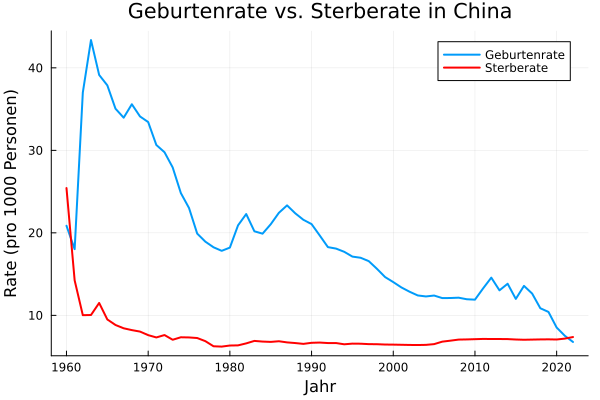
\includegraphics[width=0.6\textwidth]{geburtenrate_vs_sterberate_china.png}
    \caption{Geburtenrate vs. Sterberate in China}
    \label{fig:geburtenrate_vs_sterberate_china}
\end{figure}

Man erkennt deutlich, dass die Geburtenrate in China in den letzten Jahrzehnten deutlich gesunken ist, während die Sterberate relativ stabil geblieben ist. Dies hat zu einem Rückgang des natürlichen Bevölkerungswachstums geführt. Viele Politische sowohl als auch wirtschaftliche Faktoren haben dazu beigetragen, dass die Geburtenrate in China gesunken ist. Die Ein-Kind-Politik, die seit 2015 aufgehoben wurde, zeigt hier keinen direkten Einfluss auf die Geburtenrate. 


\subsubsection{Jährliche Wachstumsrate}

Mit den Geburten- und Sterberaten können wir die jährliche Wachstumsrate berechnen. Die jährliche Wachstumsrate gibt an, wie schnell die Bevölkerung wächst oder schrumpft. Das folgende Diagramm zeigt die jährliche Wachstumsrate in China von 1960 bis 2022.

\begin{figure}[H]
    \centering
    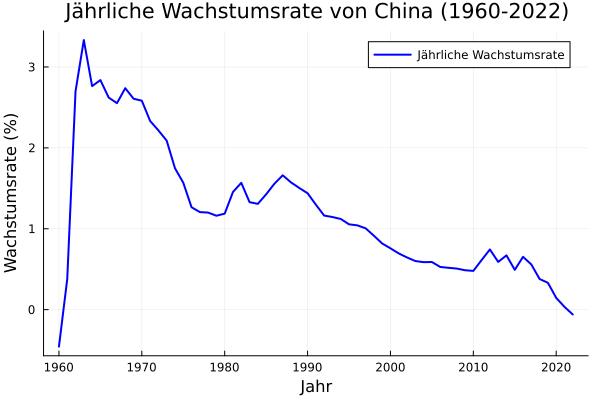
\includegraphics[width=0.6\textwidth]{jaehrliche_wachstumsrate_china_1960_2022.png}
    \caption{Jährliche Wachstumsrate von China (1960-2022)}
    \label{fig:jahreswachstumsrate_china}
\end{figure}

Deutlich zu erkennen ist, dass die jährliche Wachstumsrate in China in den letzten Jahrzehnten gesunken ist. Die sinkende Geburtenrate und die stagnierende Sterberate haben zu einem negativen Bevölkerungswachstum geführt. Im Jahr 2022 scheint die Wachstumsrate negativen Raum fortzulaufen, was auf eine schrumpfende Bevölkerung hindeutet. Mit diesen Daten können wir nun die zukünftige Bevölkerung Chinas prognostizieren.

\subsubsection{Bevölkerungsprognose}

Basierend auf den historischen Daten und den prognostizierten Wachstumsraten können wir die zukünftige Bevölkerung Chinas prognostizieren. Das folgende Diagramm zeigt die historische und prognostizierte Bevölkerung Chinas von 1960 bis 2100.

\begin{figure}[H]
    \centering
    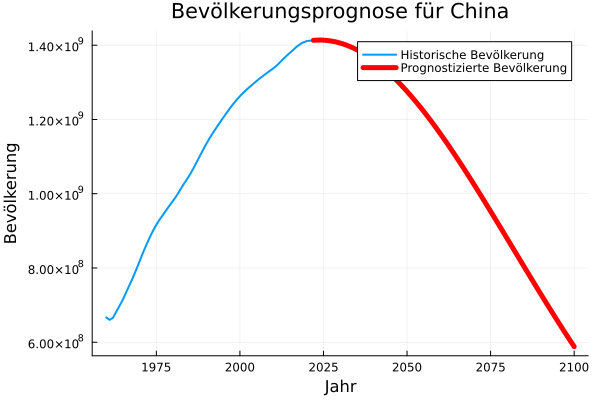
\includegraphics[width=0.6\textwidth]{bevoelkerungsprognose_china.png}
    \caption{Bevölkerungsprognose für China (1960-2100)}
    \label{fig:bevoelkerungsprognose_china}
\end{figure}

China ein Land mit knapp 1,4 Milliarden Einwohnern, wird in den nächsten Jahrzehnten wahrscheinlich eine schrumpfende Bevölkerung haben. Die Prognose zeigt, dass die Bevölkerung Chinas bis zum Jahr 2100 auf unter 1 Milliarde sinken wird. Dies hat weitreichende Auswirkungen auf die Wirtschaft, das Gesundheitswesen und die Gesellschaft Chinas. Die sinkende Bevölkerungszahl wird zu einem Rückgang der Arbeitskräfte und einem Anstieg der Altersbevölkerung führen. Dies wird die sozialen Sicherungssysteme und die Wirtschaft des Landes belasten. Die Ergebnisse der Analyse zeigen klar, dass China vor großen demografischen Herausforderungen steht, die in den kommenden Jahren bewältigt werden müssen. 

\subsection{Fazit}

Ungeachtet der politischen und wirtschaftlichen Faktoren, die die demografische Entwicklung Chinas beeinflussen, ist es wichtig, die Daten und Fakten zu verstehen, um fundierte Entscheidungen zu treffen. Die Migration und andere Faktoren wurden bei dieser Analyse nicht berücksichtigt, da sie einen geringen Einfluss auf die demografische Entwicklung Chinas haben und diese Analyse nur eine grobe Vorstellung der demografischen Entwicklung Chinas gibt. In einem Land wie China, das eine lange Geschichte und eine komplexe Gesellschaft hat, sind die demografischen Herausforderungen vielfältig und erfordern eine umfassende Strategie zur Bewältigung. Die Ergebnisse dieser Analyse können als Ausgangspunkt für weitere Untersuchungen und Diskussionen dienen, um die demografische Entwicklung Chinas besser zu verstehen und angemessene Maßnahmen zu ergreifen.

% \begin{listing}[H]
%     \begin{minted}[frame=lines, framesep=2mm, breaklines=true, baselinestretch=1.2, bgcolor=LightGray, fontsize=\footnotesize, linenos]{julia}
    
    
    
        
%     \end{minted}
%     \caption{Parameter für die Datenabfrage}
%     \end{listing}

% \inputminted[frame=lines,
% framesep=2mm,
% breaklines=true,
% baselinestretch=1.2,
% bgcolor=LightGray,
% fontsize=\footnotesize,
% linenos]{Julia}{./code/Julia4.jl}
\section{Ergebnisse}

\section{Anhang}
\inputminted[frame=lines, framesep=2mm, breaklines=true, baselinestretch=1.2, bgcolor=LightGray, fontsize=\footnotesize, linenos]{julia}{./code/Julia4.jl}
\end{document}